\documentclass[12pt,a4paper]{amsart}

% ukazi za delo s slovenscino -- izberi kodiranje, ki ti ustreza
\usepackage[utf8]{inputenc}
\usepackage[T1]{fontenc}
\usepackage[slovene]{babel}
\usepackage{lmodern} 
%\usepackage[T1]{fontenc}
%\usepackage[utf8]{inputenc}
\usepackage{amsmath,amssymb,amsfonts}
\usepackage{url}
%\usepackage[normalem]{ulem}
\usepackage[dvipsnames,usenames]{color}
\usepackage{eurosym}
\usepackage{nicefrac}
\usepackage{color}
\usepackage{hyperref}
\hypersetup{
    colorlinks=true, %set true if you want colored links
    linktoc=all,     %set to all if you want both sections and subsections linked
    linkcolor=black,  %choose some color if you want links to stand out
}

\usepackage{mathtools}
\usepackage{tikz}
\usepackage{pgfplots}
\usepackage{algorithm}
\usepackage{algorithmic}
\usepackage{caption}

% ne spreminjaj podatkov, ki vplivajo na obliko strani
\textwidth 15cm
\textheight 24cm
\oddsidemargin.5cm
\evensidemargin.5cm
\topmargin-5mm
\addtolength{\footskip}{10pt}
\pagestyle{plain}
\overfullrule=15pt % oznaci predlogo vrstico


% ukazi za matematicna okolja
\theoremstyle{definition} % tekst napisan pokoncno
\newtheorem{definicija}{Definicija}[section]
\newtheorem{primer}[definicija]{Primer}
\newtheorem{opomba}[definicija]{Opomba}

\renewcommand\endprimer{\hfill$\diamondsuit$}


\theoremstyle{plain} % tekst napisan posevno
\newtheorem{lema}[definicija]{Lema}
\newtheorem{izrek}[definicija]{Izrek}
\newtheorem{trditev}[definicija]{Trditev}
\newtheorem{posledica}[definicija]{Posledica}

\DeclareCaptionFormat{myformat}{#3}
\captionsetup[algorithm]{format = myformat}
% za stevilske mnozice uporabi naslednje simbole
\newcommand{\R}{\mathbb R}
\newcommand{\N}{\mathbb N}
\newcommand{\Z}{\mathbb Z}
\newcommand{\C}{\mathbb C}
\newcommand{\Q}{\mathbb Q}


% ukaz za slovarsko geslo
\newlength{\odstavek}
\setlength{\odstavek}{\parindent}
\newcommand{\geslo}[2]{\noindent\textbf{#1}\hspace*{3mm}\hangindent=\parindent\hangafter=1 #2}


% naslednje ukaze ustrezno popravi
\newcommand{\program}{Finančna matematika} % ime studijskega programa: Matematika/Finan"cna matematika
\newcommand{\imeavtorja}{Mitja Mandić} % ime avtorja
\newcommand{\imementorja}{izred.~prof.~dr. Jaka Smrekar} % akademski naziv in ime mentorja
\newcommand{\naslovdela}{Iterativne numerične metode v posplošenih linearnih modelih}
\newcommand{\letnica}{2021} %letnica diplome


% vstavi svoje definicije ...




\begin{document}

% od tod do povzetka ne spreminjaj nicesar
\thispagestyle{empty}
\noindent{\large
UNIVERZA V LJUBLJANI\\[1mm]
FAKULTETA ZA MATEMATIKO IN FIZIKO\\[5mm]
\program\ -- 1.~stopnja}
\vfill

\begin{center}{\large
\imeavtorja\\[2mm]
{\bf \naslovdela}\\[10mm]
Delo diplomskega seminarja\\[1cm]
Mentor: \imementorja}
\end{center}
\vfill

\noindent{\large
Ljubljana, \letnica}
\pagebreak

\thispagestyle{empty}
\tableofcontents
\pagebreak

\thispagestyle{empty}
\begin{center}
{\bf \naslovdela}\\[3mm]

{\sc Povzetek}
\end{center}
% tekst povzetka v slovenscini
V povzetku na kratko opi"si vsebinske rezultate dela. Sem ne sodi razlaga organizacije dela -- v katerem poglavju/razdelku je kaj, pa"c pa le opis vsebine.
\vfill
\begin{center}
{\bf Iterative numerical methods in generalized linear models}\\[3mm] % prevod slovenskega naslova dela
{\sc Abstract}
\end{center}
% tekst povzetka v anglescini


\vfill\noindent
{\bf Math. Subj. Class. (2010):} navedi vsaj eno klasifikacijsko oznako -- dostopne so na \url{www.ams.org/mathscinet/msc/msc2010.html}  \\[1mm]
{\bf Klju"cne besede:} navedi nekaj klju"cnih pojmov, ki nastopajo v delu  \\[1mm]
{\bf Keywords:} angle"ski prevod klju"cnih besed
\pagebreak



% tu se zacne besedilo seminarja
\section{Uvod}
Posplošeni linearni modeli so ključen del statsistične analize. Pomagajo nam bolje razumeti relacije med rezultati meritev in s temi izsledki
predvideti trende v prihodnosti. Modeli morajo biti kar se da enostavni, ampak hkrati zagotavljati določeno natančnost. Vsa teorija nam pa v praksi
ne koristi, če konkretnih številk ne znamo izračunati.

V dobi ogromne množice podatkov je računska učinkovitost ključni del obdelave. Tu nam pomagajo numerične metode.

V delu bom najprej predstavil posplošene linearne modele in najpriljubljenejše numerične metode, ki se uporabljajo za njihovo obdelavo. 
Teorijo bom osvetlil tudi s praktičnimi primeri.

\section{Eksponentna družina} 
Za uvod v nalogo si najprej definirajmo osnovo, na kateri bo kasneje temeljil eden glavnih zaključkov naloge. Predvsem nam bodo zaključki poglavja pomagali
pri posploševanju rezultatov. Slučajni vektor $Y$ torej pripada \textit{enoparametrični eksponentni družini,} če je njegova gostota oblike 
\begin{equation}
    f_{Y}(y; \theta, \phi) = \exp{\left(\frac{(y\theta - b(\theta))}{a(\phi)} + c(y, \phi)\right)},
\end{equation}
za neke funkcije $a(\cdot), b(\cdot)\text{~in~}c(\cdot).$ Če je $\phi$ znan je to eksponentna družina s \textit{kanoničnim} ali \textit{naravnim} parametrom $\theta.$

Koristno je tudi pogledati logaritem zgornje enačbe
\begin{align}
    \log f_{Y}(y; \theta, \phi) &= \frac{y\theta - b(\theta)}{a(\phi)} + c(y,\phi) \\
    \frac{\partial}{\partial \theta} \log f_{Y}(y;\theta, \phi) &= V_{\theta}(y) = \frac{(y - b'(\theta))}{a(\phi)} \\
    \frac{\partial^2}{\partial \theta^2}\ell &= -\frac{b''(\theta)}{a(\phi)},
\end{align}
kjer funkcijo $V$ imenujemo tudi \textit{funkcija zbira}, oziroma v angleščini \textit{score function.}


Dokažimo sedaj nekaj koristnih zvez, ki jih bomo uporabili v kasnejših izpeljavah.

\begin{trditev} \label{izp}
    Naj bo Y slučajna spremenljivka, katere gostota pripada eksponentni družini. Potem za pričakovano vrednost in varianco veljata sledeči zvezi:
    \[
        \mathbb{E}(Y) = b'(\theta)a(\phi),~~Var(Y) = -b''(\theta)a(\phi)
    \]
\end{trditev}
\begin{proof}
Za dokaz prve enakosti si poglejmo
\begin{align*}
    \mathbb{E}(V(y)) &= \int f_{Y}\frac{\partial}{\partial \theta}\log f_{Y}(y;\theta,\phi) \,dy = \int f_{Y}(y)\frac{1}{f_{Y}(y)}\frac{\partial f_{Y}(y)}{\partial\theta}\,dy \nonumber\\
    &=\int\frac{\partial f_{Y}(y)}{\partial \theta} \,dy= \frac{\partial}{\partial \theta}\int f_{Y}(y)\,dy = \frac{\partial}{\partial \theta}1 = 0,
\end{align*}
saj je $f_{Y}(y)$ gostota.
Od tu sledi
\begin{align*}
    \mathbb{E}(V(y)) &= \mathbb{E}(\frac{Y - b'(\theta)}{a(\phi)}) = 0 \\
    \mathbb{E}(Y) &= b'(\theta)a(\phi)
\end{align*}
Za drugo pa si oglejmo
\begin{align*}
    \mathbb{E}(\frac{\partial}{\partial\theta}V(y) - V(y)^2) &= \int f_{Y}(y)\left(\frac{\partial}{\partial \theta} \left(\frac{1}{f_{Y}(y)}\frac{\partial f_{Y}(y)}{\partial\theta}\right) + \left(\frac{\partial}{\partial\theta}\log f_{Y}(y)\right)^2\right) \,dy \\
    &= \int f_{Y}(y)\left(-\frac{1}{f_{Y}(y)^2}\left(\frac{\partial f_{Y}(y)}{\partial\theta}\right)^2 + \frac{1}{f_{Y}(y)}\frac{\partial^2f_{Y}(y)}{\partial\theta^2} + \left(\frac{1}{f_{Y}(y)}\frac{\partial f_{Y}(y)}{\partial\theta}\right)^2  \right)\,dy \\
    &=\int \frac{\partial^2}{\partial\theta^2} f_{Y}(y) \,dy = \frac{\partial^2}{\partial\theta^2}\int f_{Y}(y)\,dy = 0
\end{align*}
Spet uporabimo prej izpeljane zveze in dobimo
\begin{gather*}
    \frac{\partial^2}{\partial\theta^2}\log f_{Y}(y) = \frac{\partial}{\partial\theta}\left(\frac{y-b'(\theta)}{a(\phi)}\right) = -\frac{b''(\theta)}{a\phi},~~\mathbb{E}\left(-\frac{b''(\theta)}{a\phi}\right) = -\frac{b''(\theta)}{a\phi} \\
    \mathbb{E}\left(V(y)^2\right) = \mathbb{E}\left(\left(\frac{Y-b'(\theta)}{a(\phi)}\right)^2\right) = \frac{1}{a(\phi)^2}\mathbb{E}((Y - \mathbb{E}(Y))^2) = \frac{1}{a(\phi)^2}Var(Y),
\end{gather*}
in po zgoraj dokazani enakosti za funkcijo zbira torej velja
\begin{align*}
    -\mathbb{E}\left(\frac{\partial^2}{\partial\theta^2}f_{Y}(y)\right) &= \mathbb{E}\left(V(Y)^2\right) \\
    -\frac{b''(\theta)}{a\phi} &= \frac{1}{a(\phi)^2}Var(Y) \\
    \mathrm{Var}(Y) &= -a(\phi)b''(\theta)
\end{align*}
\end{proof}

Zgornja trditev nam torej pove, da lahko pričakovano vrednost in varianco porazdelitve iz eksponentne družine, z nekaj odvajanja, preberemo kar iz gostote - izognemo se integriraciji. Po drugi
strani pa vidimo, da je varianca le funkcija pričakovane vrednosti. 

Pričakovano vrednost kvadrata funkcije zbira v splošnem imenujemo \textit{Fisherjeva informacija}, $FI(\theta) = E((V(Y))^2),$ izpeljano zvezo, ki poveže funkcijo zbira in njene odvode pa \textit{informacijska enakost.}
Uporabnost teh zvez bo postala jasna v sledečih poglavjih.

Oglejmo si sedaj nekaj primerov porazdelitev eksponentne družine:
\begin{itemize}
    \item \textbf{Normalna porazdelitev.} Normalno porazdeljena slučajna spremenljivka $Y \sim N(\mu, \sigma^2)$
    ima gostoto $f_{Y}(y) = \frac{1}{\sqrt{2\pi\sigma^2}}\exp{\left(-\frac{(y-\mu)^2}{2\sigma^2}\right)}.$
    Če zgornjo enačbo logaritmiramo dobimo
    \begin{align*}
        \log f_{Y}(y;\mu, \sigma) &= \log\left(\frac{1}{\sqrt{2\pi\sigma^2}}\right) -\frac{(y-\mu)^2}{2\sigma^2} = -\frac{1}{2}\log(2\sigma^2\pi) - \frac{y^2 - 2\mu y + \mu^2}{2 \sigma^2}    \\ \nonumber
                            &= \frac{y\mu-\nicefrac{\mu^2}{2}}{\sigma^2} - \frac{1}{2}\left(\frac{y^2}{\sigma^2} + \log(2\pi\sigma^2)\right) 
    \end{align*}
    Od tu preberemo zgoraj definirane vrednosti
    \[
        \theta = \mu,~a(\phi) = \sigma^2,~b(\theta) = \frac{\theta^2}{2}
    \]
    in takoj sledijo zaključki
    \[
        \mathbb{E}(Y) = b'(\theta) = \mu \text{ in } \mathrm{Var}(Y) = a(\phi)b''(\theta) = \sigma^2,
    \]
    kar se ujema z zvezami iz trditve \ref{izp}.

    \item \textbf{Binomska porazdelitev.} Imejmo binomsko porazdeljen slučajni vektor $Y \sim \mathrm{Bin}(n,p).$ Verjetnost 
    \[
        \mathrm{P}(Y = y) = \binom{n}{y}p^y(1-p)^{n-y} = \exp\left(y\log(\frac{p}{1-p}) + n\log(1-p) + \log{\binom{n}{k}}\right),
    \]
    od koder direktno sledi
    \[
        \theta = \log\frac{p}{1-p},~b(\theta) = n\log(1 + e^{\theta}),~a(\phi) = 1,
    \]
    in opazimo da je tokrat naravni parameter $\log\frac{1}{1-p},$ kar imenujemo tudi \textit{logit} verjetnosti. Pomembnost tega rezultata 
    bomo videli v naslednjih poglavjih.
\end{itemize}

Poleg omenjenih, spadajo v eksponentno družino še Gamma, $\chi^2,$ eksponenta, Poissonova in kar nekaj drugih porazdelitev.
\section{Posplošeni linearni modeli}

\subsection{Sestavni deli posplošenega linearnega modela}
Vsak posplošeni linearni model sestavljajo trije deli: \textit{slučajni del} je slučajna spremenljivka $Y$ in njena porazdelitev, 
\textit{sistematični del} predstavlja relacijo med pojasnjevalnimi spremenljivkami, \textit{povezovalna funkcija} pa transformira $E(Y)$, da se ta
bolje prilega podatkom.

\subsubsection{Slučajni del}
\textit{Slučajni del} privzame porazdelitev slučajnega vektorja $Y$, pri čemer privzemamo tudi neodvisnost komponent. Porazdelitev $Y$
privzemamo odvisno od podatkov; mnogokrat je ,,binarna``, torej ima dve možni vrednosti - ,,uspeh`` ali ,,neuspeh``. Splošneje je lahko izid tudi 
število uspehov v fiksnem številu poskusov. V takih primerih privzamemo binomsko porazdelitev. $Y$ nam lahko meri tudi števne podatke, naprimer 
koliko zabav je obiskal študent v preteklem mesecu. Seveda pa lahko $Y$ predstavlja tudi zvezne podatke,
v tem primeru lahko privzamemo normalno porazdelitev (ali pa kakšno drugo zvezno porazdelitev).
\subsubsection{Sistematični del} 
\textit{Sistematična komponenta} posplošenega linearnega modela poda relacije med pojasnjevalnimi spremenljivkami $x_{ij}$. Te nastopajo 
linearno, torej je sistematični del enak
\[
\beta_{0} + x_{i1}\beta_{1} + x_{i2}\beta_{2} + \ldots + x_{ip}\beta_{p}
\]
\subsubsection{Povezovalna funkcija}
Tretji del posplošenega linearnega modela je \textit{povezovalna funkcija}, ta nam poda funkcijo $g(\cdot)$ med slučajno komponento
in sistematičnim delom. Če označimo $\mu = E(Y)$, je
\[
    g(\mu) = \beta_{0} + x_{i1}\beta_{1} + x_{i2}\beta_{2} + \ldots + x_{ip}\beta_{p}
\]
Najenostavnejša taka funkcija je kar identiteta, torej $g(\mu) = \mu$. Ta nam torej da linearno povezavo med pojasnjevalnimi spremenljivkami 
in pričakovano vrednostjo naših slučajnih spremenljivki. To je ena od oblik regresije za zvezne podatke.
Mnogokrat pa linearna relacija ni primerna - fiksna sprememba pojasnjevalnih spremenljivk ima lahko večji vpliv, če je pričakovana vrednost 
bližje 0, kot če je bližje 1. Recimo, da je $\pi$ verjetnost, da bo oseba kupila nov avto, ko je njen dohodek enak $x$. Sprememba v dohodku
za 10.000\euro~ima manjši vpliv, če je dohodek 1.000.000\euro,~kot če je 50.000\euro.
Takrat je smiselno uporabiti kakšno drugo povezovalno funkcijo, ki dopušča tudi nelinearne kombinacije pojasnjevalnih
spremenljivk. Naprimer, $g(\mu) = \log(\mu)$ modelira
pričakovano vrednost logaritma. Smiselno jo je uporabiti, če pričakovana vrednost ne more zavzeti negativnih vrednosti. Takemu modelu rečemo
\textit{log-linearen} model.
Spet druga povezovalna funkcija je $\mathrm{logit}(\mu) = \log(\frac{\mu}{1-\mu})$, ki nam modelira logaritem deležev - smiselno jo je uporabiti, 
ko $\mu$ ne zavzame vrednosti izven $(0,1)$, torej ko imamo opravka z verjetnostmi. Takemu modelu rečemo logistični model.
%\subsection{Primeri posplošenih linearnih modelov}
\subsection{Točkovno ocenjevanje}
Preden se natančneje posvetimo posplošenim linearnim modelom, si oglejmo dve najbolj znani metodi za ocenjevanje parametrov.
Najprej si definirajmo nekaj pojmov, ki jih bomo uporabljali v nadaljnjih poglavjih.

\textit{Cenilka} za realnoštevilsko karatkreristiko $c$ proučevane porazdelitve je funkcija vzorca $T=T(X_{1},\ldots,X_{n})$, s katero ocenjujemo $c.$
Ta cenilka je \textit{nepristranska}, če za porazdelitev vzorca $F$ velja $E(T(X_{1},\ldots,X_{n})) = c(F).$
Imejmo sedaj zaporedje cenilk za vzorce velikosti $n=1,2,\ldots.$ To zaporedje je \textit{dosledno}, če v verjetnosti konvergira h konstanti $c(F).$

Če povzamem z drugimi besedami; nepristranska cenilka nam v povprečju vrne pravi rezultat, dosledna cenilka pa z večjim vzorcem vrne rezultat vedno
bližje ocenjevani karakteristiki.

\subsubsection{Metoda momentov}
Metodo momentov je Čebišev leta 1887 predstavil v svojem dokazu centralnega limitnega izreka. V splošnem ni tako uporabna kot spodaj opisana metoda največjega
verjetja, je pa precej enostavna za računanje brez računalnika. Po besedah profesorja Smrekarja iz predavanj Verjetnosti in statistike\:
,,metoda momentov sloni na filozofiji: vse kar se da izraziti z momenti, izrazimo z momenti.``

V splošnem z metodo momentov postopamo takole: če je ocenjevano karakteristiko proučevane slučajne spremenljivke $c(X)$ mogoče izraziti kot funkcijo 
momentov,t.j. če v danem modelu ti momenti obstajajo, 
\[
    c(X) = g(m_{1}(X), m_{2}(X),\ldots,m_{r}(X)),
\] za neko funkcijo g, potem $c(X)$ ocenjujemo s cenilko $g(\hat{m}_{1},\ldots,\hat{m}_{r}).$ Če je g zvezna, dobimo dosledno cenilko.

\subsubsection{Metoda največjega verjetja}
Imejmo parametrični model s prostorom parametrov $\Theta \subseteq \mathbb{R}^{r}$ in pripadajoč vektorski parameter $\theta = (\theta_{1},\ldots,\theta_{r}).$
Privzemimo, da imajo vse proučevane porazdelitve gostote oziroma verjetnostne funkcije oblike
\[
    f(x;\theta) = f(x;\theta_{1},\ldots,\theta_{r}).
\]
Funkcijo verjetja za vzorec velikosti $n$ definiramo kot funkcijo paramtetra $\theta$, in sicer
\[
    F(X_{1},\ldots,X_{n};\underbrace{\theta_{1},\ldots,\theta_{r}}_{\theta}) = f(X_{1},\theta)\cdots f(X_{n},\theta).
\]
Kot funkcija vektorja $x$ pa je $F$ gostota slučajnega vektorja $X = (X_{1},\ldots,X_{n}).$

Najti želimo tak parameter, v katerem bo funkcija verjetja zavzela svoj maksimum, torej 
\[
    F(\hat{\theta}) = \underset{\theta \in \Theta}{\max}{F(\theta)}.
\]
Opazimo, da si računanje lahko precej poenostavimo, če obe strani zgornje enačbe logaritmiramo
\begin{equation}
    \log(F(\theta)) = L(\theta) = \sum_{i=1}^{n}\log f(x_{i},\theta).
\end{equation}
Funkciji $L$ rečemo logaritemska funkcija verjetja, njene stacionarne točke pa bodo kandidati za cenilko največjega verjetja. Ker je logaritem 
naraščajoča funkcija, bodo ekstremi $L$ in $F$ sovpadali. Rešiti moramo torej sistem enačb
\begin{equation}\label{mle}
    \frac{\partial}{\partial \theta_{j}}(L(\theta)) = 0~,j=1,\ldots,r,
\end{equation}
ki mu rečemo tudi sistem \textit{enačb verjetja}, odvod logaritemske funkcije verjetja pa v statistiki pogosto poimenujejo \textit{zbirna funkcija}.
Ko rešimo enačbe verjetja, najdemo ekstrem funkcije verjetja in dobimo \textit{cenilko največjega verjetja}, v angleščini pogosto označeno MLE (okrajšava za
\textit{maximum likelihood estimator}).

Tako dobljene cenilke niso nujno nepristranske, so pa dosledne, če je rešitev \eqref{mle} enolična. V splošnem take enačbe niso rešljive eksplicitno, zato se poslužujemo različnih
numeričnih metod za njihovo reševanje. Nekatere so predstavljene v drugem delu naloge.

\subsection{Linearna regresija}
Linearna regresija je najenostavnejši primer posplošenega linearnega modela. Enostavno jo lahko zapišemo kot:
$
    Y = X \beta + \varepsilon
$
kjer je $Y$ proučevan slučajni vektor, $X$ je matrika pojasnjevalnih slučajnih spremenljivk, $\beta$ je vektor koeficientov, ki jih želimo oceniti,
$\varepsilon$ pa slučajna spremenljivka, ki predstavlja napako - pri računanju, meritvah \ldots. Privzemimo, da je $E(\varepsilon) = 0$. Iz tega sledi
$\mu = E(Y) = X\beta$. Model torej pričakovano vrednost slučajne spremenljivke predstavi kot linearno funkcijo pojasnjevalnih spremenljivk.
Parametre $\beta$ ocenimo z metodo najmanjših kvadratov in ob predpostavki polnega ranga za matriko $X$ dobimo $\hat{\beta} =  (X^\top X)^{-1}
X^\top y$, kjer smo do slednjega sistema enačb prišli preko pretvorbe na normalni sistem enačb. Ko rešimo ta sistem, dobimo zgoraj opisano cenilko največjega verjetja-

%\subsection{Poissonova regresija}

\subsection{Logistična regresija}
Logistična regresija se uporablja za določanje deležev oziroma računanje verjetnosti. V poštev pride, ko imamo odgovore tipa uspeh-neuspeh oziroma
govorimo o prisotnosti ali odsotnosti neke lastnosti.
Spomnimo se Binomske porazdelitve $Y_{i} \sim B(n_{i}, p_{i})$. Ta pravi, da je 
\[
    P(Y_{i} = y_{i}) = {n_{i} \choose y_{i}} p_{i}^{y_{i}}(1 - p_{i}) ^{n_{i} - y_{i}}
\]
Pričakovana vrednost in varianca sta odvisni le od $p_{i}$, in sta enaki $E(Y_{i}) = n_{i}p_{i} \text{~in}\\Var(Y_{i}) = n_{i}p_{i}(1 - p_{i}).$~
Poglejmo si sedaj podrobneje \textit{logit} transformacijo. Če se spomnemo, želimo določiti verjetnost nekega dogodka pri danih podatkih. Ob uporabi
identitente transformacije se nam kaj hitro lahko zgodi, da za posamezne verjetnosti dobimo vrednosti izven intervala $[0,1]$. Ta problem bomo rešili v 
dveh korakih.
Najprej uvedimo 
\[ 
    \mathrm{dele"z}_{i} = \frac{p_{i}}{1 - p_{i}} %poglej kako se tle da vejico
\]
kjer se premaknemo iz verjetnosti v \textit{deleže} -- verjetnost dogodka proti verjetnosti, da se ne bo zgodil. Če je $p_{i}$ enak $\frac{1}{2}$, 
bo delež enak 1. Vidimo, da so deleži vedno pozitivni in niso omejeni navzgor.
V naslednjem koraku pa poglejmo logaritem deležev ali logit verjetnosti
\[
    \eta_{i} = \mathrm{logit}(p_{i}) = \log \frac{p_{i}}{1 - p_{i}}
\]
s tem pa si odstranimo tudi omejitev navzdol. Opazimo še, da če je $p_{i} = \frac{1}{2}$, je delež enak 1 in je logaritem 0. Kot funkcija p, je logit
strogo naraščajoča, torej imamo inverz. Običajno ga imenujemo \textit{antilogit}, izrazimo ga z:
\[
    p_{i} = \mathrm{logit}^{-1}(\eta_{i}) = \frac{\exp{\eta_{i}}}{1+\exp{\eta_{i}}} = \frac{\exp{x_{i}^\top\beta}}{1+\exp{x_{i}^\top\beta}}
\]
Vse skupaj nam da \textit{logistični model}, ki za slučajni del vzame binomsko porazdelitev. %VPRAŠAJ KAJ JE Z NAPAKO
Kot vidimo, zveza med prediktorji in verjetnostjo ni linearna, zato je težko oceniti, kako bo sprememba parametrov
vplivala na verjetnost. Na to vprašanje lahko približno odgovorimo tako, da odvajamo po spremenljivki $x_{j}$ (kar ima seveda smisel le za zvezne
pojasnjevalne spremenljivke) in dobimo $\nicefrac{\partial}{\partial x_{j}} = \beta_{j}p_{i}(1 - p_{i}).$~Vidimo, da na spremembo j-tega prediktorja
vpliva tako verjetnost kot tudi parameter $\beta$. Običajno se za analizo vzame vzorčno povprečje verjetnosti opazovane vrednosti.
\subsubsection{Ocenjevanje parametrov}\label{ocenpar}
Imamo binomske slučajne spremenljivke in imamo povezovalno funkcijo, $\mathrm{}{logit p_{i}} = X\beta$, kjer so $\beta$ neznani parametri.
V naslednjem razdelku si bomo ogledali kako zanje izpeljemo enačbe verjetja, ki jih nato uporabimo v numeričnih algoritmih.
Kot v vsakem posplošenem linearnem modelu tudi v tem predpostavimo neodvisnost komponent slučajnega vektorja $\mathrm{Y}$ zato 
\begin{align*}
    P(Y = \vec{y}) &= \prod_{i=1}^{n} P(Y_{i} = y_{i}) \\
                    &=\prod_{i=1}^{n} {n_{i} \choose y_{i}} p_{i}^{y_{i}}(1 - p_{i})^{n_{i} - y_{i}}
\end{align*}
Naprej si oglejmo logaritemsko funkcijo verjetja. V nadaljnem računanju bom izpuščal binomski simbol na začetku - je samo konstanta, ki na
končen rezultat nima vpliva. Po prejšnjih oznakah je torej
\begin{align}\label{logit1}
    L(p_{i}) &= \log\{\prod_{i=1}^{n} p_{i}^{y_{i}}(1 - p_{i})^{n_{i} - y_{i}} \} \nonumber  \\
        &= \sum_{i=1}^{n}\{y_{i}\log{p_{i}} + (n_{i} - y_{i})\log(1 - p_{i})\} \nonumber \\
        &= \sum_{i=1}^{n}\{n_{i}\log{(1-p_{i})}  + y_{i}\log{\left(\frac{p_{i}}{1-p_{i}}\right)}\}
\end{align}
Po predpostavki logističnega modela je 
\[
   \mathrm{logit}(p_{i}) = \log\left( \frac{p_{i}}{1-p_{i}}  \right) = \beta_{0} + x_{i1}\beta_{1} + \ldots + x_{ir}\beta_{r} = x_{i}^\top \beta,
\]
iz česar lahko izrazimo verjetnost $p_{i}$
\begin{align}
    p_{i} &= \frac{\exp{x_{i}^{\top} \beta}}{1 + \exp{x_{i}^\top\beta}} \text{~ter} \\
    1 - p_{i} &= \frac{1}{1 + \exp{x_{i}^\top\beta}}
\end{align}

\pagebreak
Zgornji funkciji rečemo \textit{sigmoida}. Iz njenega grafa je morda še bolj očitno, zakaj jo je smiselno uporabiti za modeliranje verjetnosti
\begin{center}
\begin{figure}[h]
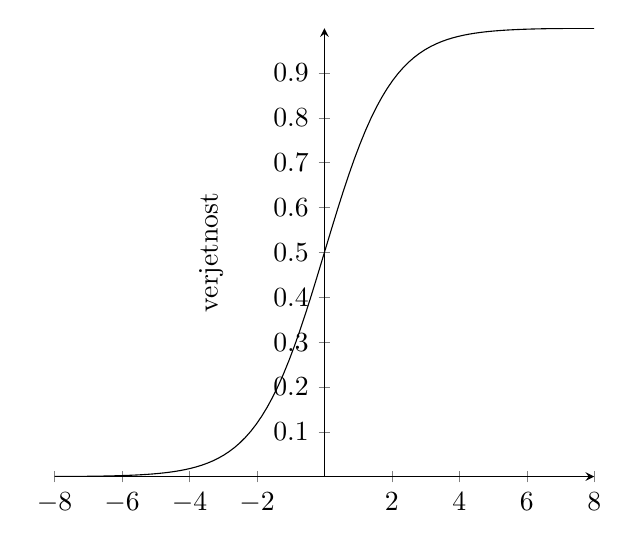
\begin{tikzpicture}
    \begin{axis}[
        axis lines = center,
        %xtick = {-10,-9,-8,...,9,10}
        ytick = {0,0.1,0.2,...,0.9,1},
        ylabel = verjetnost,
        y label style = {at={(axis description cs:0.25,.5)},rotate=90}%,anchor=south}
    ]
    \addplot [
        domain=-8:8, 
        samples=100, 
        color=black,
        ]
        {exp(x)/(1+exp(x))};
    %\addlegendentry{$x^2 + 2x + 1$}
    
    \end{axis}
\end{tikzpicture}
\caption{Graf sigmoide}
\label{fig:sigmoid}
\end{figure}
\end{center}

Če izpeljane izraze za verjetnost upoštevamo v logaritemski funkciji verjetja dobimo
\begin{align}
    \ell(\beta) &= \sum_{i=1}^{n}\left( n_{i}\log{\frac{1}{1 + \exp{x_{i}^\top\beta}}}  + y_{i}\log{\left( \frac{\frac{\exp{x_{i}^{\top} \beta}}{1 + \exp{x_{i}^\top\beta}}}{\frac{1}{1 + \exp{x_{i}^\top\beta}}}  \right)} \right) \nonumber\\
                &= \sum_{i=1}^{n}\left( y_{i}(x_{i}^\top\beta) - n_{i}\log(1 + \exp{x_{i}^\top\beta})           \right)
\end{align}
Od tod vidimo, da je naša funkcija verjetja zares odvisna le od parametrov $\beta$,~vse ostalo nam je poznano. Da torej poiščemo maksimum in s tem
cenilko največjega verjetja, funkcijo odvajamo in zbirno funkcijo enačimo z 0
\[
    \dot{\ell}(\beta) = \begin{bmatrix}
                                 \frac{\partial \ell(\beta)}{\partial \beta_{0}} \\
                                 \frac{\partial \ell(\beta)}{\partial \beta_{1}} \\
                                 \vdots \\
                                 \frac{\partial \ell(\beta)}{\partial \beta_{p}}
                        \end{bmatrix}
\]
Pomembno je opaziti, da parametri $\beta$ vedno nastopajo ob pojasnjevalnih spremenljivkah linearno -- zato bodo komponente zbirne funkcije simetrične.
J-ta komponenta bo tako enaka
\begin{align}
    \frac{\partial \ell(\beta)}{\partial \beta_{j}} &= \sum_{i=1}^{n} \left(x_{ij}(y_{i} - n_{i}p_{i}(\beta))   \right),~~j = 0,1,\ldots r,~~\text{kjer~smo~upoštevali} \\
    \frac{\partial}{\partial \beta_{j}}(x_{i}^\top\beta) &= \frac{\partial}{\partial \beta_{j}}\left(\beta_{0} + x_{i1}\beta_{1} + \ldots x_{ir}\beta_{r}\right) \nonumber\\
                                                    &= x_{ij},
\end{align}
ter
\begin{align}                                         
    \frac{\partial}{\partial \beta_{j}} \log(1 + \exp(x_{i}^\top\beta)) &= \frac{ \frac{\partial}{\partial \beta_{j}}\exp(x_{i}^\top\beta) }{1 + \exp(x_{i}^\top\beta)} \nonumber \\
    &= \frac{\exp(x_{i}^\top\beta)}{1 + \exp(x_{i}^\top\beta)} \frac{\partial}{\partial \beta_{j}} (x_{i}^\top\beta) \nonumber \\
    &=p_{i}(\beta)x_{ij}
\end{align}
Enačbe, ki jih s tem postopkom dobimo, v splošnem niso eksplicitno rešljive. Za reševanje se uporablja numerične metode, ki slonijo na Newtonovi iteraciji. Kot
bomo kasneje pokazali, je zanjo potrebno izračunati še drugi odvod, zato to storimo tu. Zopet odvajamo po komponentah, tako kot zgoraj. Najprej izračunajmo
\begin{align}
    \frac{\partial p_{i}(\beta)}{\partial \beta_{k}} &= \frac{\partial}{\partial \beta_{k}} \frac{\exp{x_{i}^\top\beta}}{1+\exp{x_{i}^\top\beta}} \nonumber \\
        &= x_{ik}p_{i}(\beta)(1 - p_{i}(\beta)) \nonumber
\end{align}
Vse sedaj skupaj sestavimo v
\begin{align}
    \frac{\partial^2}{\partial \beta_{j}\partial\beta_{k}} \ell(\beta)= - \sum_{i}^{n}\left(x_{ij}x_{ik}n_{i}p_{i}(\beta)(1-p_{i}(\beta))\right),~~j,k = 0,1,\ldots, r
\end{align}
Spomnimo se, da delamo z binomskimi slučajnimi spremenljivkami in torej velja $var(Y_{i}) = v_{i}(\beta) = n_{i}p_{i}(1-p_{i}),$~kar vključimo v zgornjo enačbo in končno dobimo
\begin{align}
    \ddot{\ell}(\beta) = -\sum_{i=1}^{n}\left(x_{ij}x_{ik}v_{i}(\beta)\right).
\end{align}
Zapišimo zgoraj izpeljane zveze v berljivejšo matrično notacijo. 
\begin{equation*}
    \log \left(\frac{p}{1-p}\right) = \mathbf{X}\beta
\end{equation*}
Vektorsko definiramu tudi
\[
    \exp{\mathbf{X}\beta} = \begin{bmatrix}
                            \exp{x_{1}^\top\beta} \\
                            \vdots\\
                            \exp{x_{n}^\top\beta}
                            \end{bmatrix},
\]
spomnimo se enačbe \eqref{logit1} in iz nje izpeljimo %DOPOLNI KER NI NITI MALO JASNO OD KOD TO PRIDE
\begin{align} \label{ell}
    \ell(\beta) &= \sum_{i=1}^{n}\{n_{i}\log{1-p_{i}}  + y_{i}\log{\left(\frac{p_{i}}{1-p_{i}}\right)}\} \nonumber\\
    &= y^\top\mathbf{X}\beta - n^\top \log(1 + \exp{\mathbf{X}\beta}),
\end{align}
in še odvoda zgornje funkcjie, ki pa ga lahko zapišemo kot
\begin{equation}
    \dot{\ell}(\beta) = \mathbf{X}^\top(y - m\circ p(\beta)),
\end{equation}
kjer je s $\circ$ označeno Hadamardovo množenje po elementih.
S pričakovano vrednostjo vektorja označimo vektor pričakovanih vrednosti komponent in torej lahko zapišemo
\begin{equation}
    \mathrm{E}(Y) = m \circ p(\beta) \equiv \mu(\beta),
\end{equation}
in lahko končno vse povzamemo v
\begin{align}\label{prvi}
    \dot{\ell}(\beta) = \mathbf{X}^\top(y - m \circ p(\beta)) = X^\top(y - \mu(\beta))
\end{align}
Ostane nam le še dvojni odvod. Najprej si oglejmo
\[
    v(\beta) = \begin{bmatrix}
        v_{1}(\beta)  & & &\\
        & v_{2}(\beta) & & \\
        & & \ddots & \\
        & & & v_{n}(\beta)
    \end{bmatrix},
\]
iz tega potem takoj sledi, da je
\begin{equation} \label{drugi}
    \ddot{\ell}(\beta) = -\mathbf{X}^\top v(\beta)\mathbf{X},
\end{equation}
torej element v $j$-ti vrstici in $k$-tem stolpcu je $\sum_{i=1}^{n}x_{ij}x_{ik}v_{i}(\beta).$

\subsection{Kanonični modeli v splošnem}
Kot bomo spoznali v sledečem razdelku, spada logistična regresija med tako imenovane modele s "'kanonično"` povezovalno funkcijo. 
Za vpeljavo tega ter prenekaterih ostalih pojmov pa potrebujemo nekaj dodatne teorije.

\subsubsection{Kaj so kanonične povezovalne funkcije?}
Kot smo omenili že v uvodu povezovalna funkcija opisuje relacijo med pričakovano vrednostjo opazovane spremenljivke in desno stranjo našega modela, torej
sistematično komponento modela. Eksponentno družino torej v splošnem sestavljajo porazdelitve, z gostotami oblike
\[
    f_{Y}(y; \theta, \phi) = \exp{\left(\frac{(y\theta - b(\theta))}{a(\phi)} + c(y, \phi)\right)}.
\]
Enačbo logaritmiramo in dobimo
\[
    L(y;\theta) = \frac{y\theta-b(\theta)}{a(\phi)} + c(y;\phi),
\]
njen odvod, torej funkcija zbira pa je 
\[
    \frac{\partial}{\partial \theta} L(y;\theta) = \frac{y-b'(\theta)}{a(\phi)}.
\]
O kanonični povezovalni funkciji govorimo, če velja $\theta=\eta,$ torej je naravni parameter eksponentne družine ravno enak funkciji pričakovane vrednosti v modelu.
Da uporabimo logit verjetnosti v logističnem modelu torej ni naključje - videli smo, da je $\textbf{logit}(p_{i})$ enak parametru $\theta.$ Spodaj je navedenih še nekaj ostalih
kanoničnih povezovalnih funkcij, njihovo uporabnost bomo spoznali v naslednjem razdelku.

\begin{center}
    \begin{tabular}{ | c | c | c |}
        \hline
        Porazdelitev & $f(\mu)$ & Uporaba \\
        \hline
        Normalna & $id(\mu)$ &  Linearni odgovori\\
        Poissonova & $\log \mu$ & Število pojavitev \\
        Binomska & $\mathrm{logit}\mu$ & Binarni podatki\\
        Gamma & $-\frac{1}{\mu}$ & \\
        \hline
    \end{tabular}
\end{center}

\subsection{Probit regresija}
Probit regresija se uporablja v podobne namene kot logistična, torej za določanje verjetnosti in razvrščanje. Razvili so jo v tridesetih letih
dvajsetega stoletja, ime pa je skovanka -- pride iz angleških besed \textit{\textbf{prob}ability un\textbf{it}}. V glavnem se od logistične regresije
razlikuje v sistematičnem delu. Verjetnost pozitivnega izida torej po modelu predpostavljamo
\begin{equation}
    p_{i}(\beta) = \Phi (\beta_{0} + x_{i1}\beta_{1} + \ldots + x_{ir}\beta_{r}),
\end{equation}
kjer $\Phi$ predstavlja kumulativno porazdelitveno funkcijo standardne normalne slučajne spremenljivke. Ta seveda ni linearna (v nasprotju s prejšnjimi modeli),
podana je kot 
\[
    \Phi(x) = \frac{1}{\sqrt{2\pi}}\int_{-\infty}^{x}e^{\frac{-t^2}{2}}\,dt
\]

\subsubsection{Ocenjevanje parametrov probit regresije}
Podobno kot v logističnem modelu, se bomo ocenjevanja parametrov lotili po metodi največjega verjetja. 

Za sistematični del modela privzemimo binomsko porazdeljene slučajne spremenljivke s parametroma $B(m_{i},p_{i}(\beta))$,
verjetnost pozitivnega izida pa izrazimo z
\[
    P(Y_{i} = y_{i}) = \binom{m_{i}}{y_{i}}p_{i}(\beta)^{y_{i}}(1 - p_{i}(\beta))^{m_{i} - y_{i}} = \binom{m_{i}}{y_{i}} (\Phi(x_{i}^\top \beta)^{y_{i}})(1 - \Phi(x_{i}^\top \beta))^{m_{i} - y_{i}} 
\]
Funkcijo verjetja, tako kot zgoraj izrazimo z gostotami posameznih komponent
\[
    \ell(\beta) = \prod_{i=1}^{n} \binom{m_{i}}{y_{i}} \Phi(x_{i}^\top\beta)^{y_{i}}(1 - \Phi(x_{i}^\top\beta))^{m_{i} - y_{i}},
\]
kjer binomski simbol izpustimo zaradi enostavnejšega pisanja. Zgornjo enačbo logaritmiramo in dobimo
\begin{equation}
    \log(\ell(\beta)) = L(\beta) = \sum_{i = 1}^{n}\left(y_{i}\log\Phi(x_{i}^\top\beta) + (m_{i} - y_{i})\log(1 - \Phi(x_{i}^\top\beta)) \right)
\end{equation}
Enačbo zopet odvajamo po parametru $\beta,$ vendar se nam v tem primeru ne poenostavi kot z logistično funkcijo.

\subsection{Ne-kanonični modeli v splošnem}

\section{Numerične metode}
V sledečih razdelkih si bomo od bliže pogledali nekaj numeričnih metod, uporabljenih v kasnejših zgledih. Te metode slonijo na stoletja starih
idejah, ki smo jih spoznali tekom študija, uporabljajo pa se tudi v številnih praktičnih aplikacijah.
\subsection{Newton -- Raphsonova metoda} \label{nr}
Newton -- Raphson (oziroma le Newtonova) metoda je bila v osnovi razvita za iskanje ničel funkcije. Spada v razred \textit{navadnih iteracij}, torej metod za iterativno
reševanje enačb $f(x) = 0,$ ki jih prevedemo na $g(x) = x,$ izberemo začetni približek $x_{0}$ in ponavljamo 
\[
    x_{r+1} = g(x_{r}).
\]

V najosnovnejši (ter najpogostejši) verziji za iskanje
ničle funkcije ene spremenljivke začnemo v neki točki, naslendnjo pa izberemo v presčišču tangente, izračunane v 
tej točki, z x-osjo. Postopek tako iterativno nadaljujemo. Ideja je torej sila preprosta, za izpeljavo pa tudi ni potrebno preveč truda.
Predpostavimo odvedljivost funkcije na nekem intervalu in recimo, da imamo trenuten približek $x_{n}.$~Razvijmo sedaj funkcijo v Taylorjev
polinom prve stopnje okoli $x_{n}:$
\[
    f(x) \approx f(x_{n}) + f'(x_{n})(x - x_{n})
\]
Presečišče najdemo, če zgornjo enačbo enačimo z 0 in dobimo znano formulo
\[
    x_{n+1} = x_{n} - \frac{f(x_{n})}{f'(x_{n})}.
\]
Metoda bo skonvergirala za začetne približke dovolj blizu ničli in v neki okolici ničle konvergirala s kvadratično hitrostjo. 
Na težave naletimo v več primerih. Najprej, blizu stacionarne točke metoda odpove, saj bi delili z 0 (oziroma vrednostmi blizu ničle, kar je numerično nestabilno).
Problem lahko predstavlja tudi računanje odvoda, ki zna biti zahtevno, ter dejstvo, da za slabe začetne približke ničle morda ne bomo našli. S temi 
težavami se bomo soočili v nadaljevanju.
Imamo torej algoritem, ki najde ničlo, v luči iskanja cenilke največjega verjetja pa bi želeli algoritem, ki poišče maksimum oziroma minimum funkcije.
Recimo, da imamo neko logaritemsko funkcijo verjetja $L$, in trenutni približek $\theta_{n}$. Razvijmo funkcijo okoli približka v Taylorjev polinom
druge stopnje:
\begin{align}
    L(\theta) \approx L(\theta_{n}) + dL(\theta_{n})(\theta - \theta_{n}) + \frac{1}{2}(\theta - \theta_{n})^\top d^{2}L(\theta_{n})(\theta - \theta_{n}) \label{taylor}   
\end{align}
Maksimizirati želimo desno stran \eqref{taylor}. To storimo tako, da gradient $L$ enačimo z nič:
\[
    \nabla L(\theta_{n}) + \nabla^2L(\theta_{n})(\theta - \theta_{n}) = 0  
\]
in izrazimo naslednji približek
\[
    \theta_{n + 1} = \theta_{n} - \nabla^{2}L(\theta_{n})^{-1}\nabla L(\theta_{n}).
\]
S tem postopkom imamo lahko dva problema. Prvič, lahko je zahtevno računati in invertirati drugi odvod (Hesian) funkcije, morda za kakšen $\theta_{n}$ sploh ne obstaja.
Drugič, proč od $\hat{\theta}$ lahko Newtonova metoda napreduje navzgor ali navzdol -- oboje je enako verjetno. Z drugimi besedami, Newtonova metoda ni naraščajoč algoritem in torej
ne da $L(\theta_{n}) < L(\theta_{n+1}).$ Mi pa bi želeli algoritem, ki bo konvergiral globalno (in ne le na nekem intervalu okoli rešitve).
Težavo z računanjem inverza rešimo tako, da namesto invertiranja problem prevedemo na reševanje sistema enačb za premik:
\begin{align}\label{newtoneq}
    x_{n + 1} &= x_{n} + p_{n} \nonumber\\
    \nabla^2L(\theta_{n})p_{n} &= -\nabla L(\theta_{n})
\end{align}
Zadnji vrstici v \eqref{newtoneq} rečemo tudi \textit{Newtonova enačba}.
Radi bi še dosegli, da bi se Newtonov algoritem premikal v eno smer, torej naraščal ali padal. S tem bi vedeli, kaj se bo zgodilo v iteraciji in lažje predvideli morebitne
nevšečnosti. Newtonova metoda za iskanje minimuma (maksimum) funkcije je optimizacijski problem drugega reda in realna funkcija ima globalni minimum (maksimum) tam, kjer je
njen drugi odvod pozitiven, oziroma v primeru funkcij več spremenljivk, kjer je njen Hesian pozitivno definiten (in je tam gradient enak nič). Če bi torej imeli
strogo pozivino definitno matriko, bi bil ta optimizacijski problem konveksen in kot tak rešljiv globalno (veljati morajo še pogoji Karush-Kuhn-Tuckerja, vendar je to skoraj vedno res).
Imejmo torej v točki $x^{*}$ pozitivno definitno Hessejevo matriko $H.$~Zapišimo Taylorjev polinom druge stopnje okoli te točke
\[
    f(x^{*} + s) = f(x_x^{*}) + \nabla f(x^{*})s + \frac{1}{2}s^\top H(x^{*})s.
\]
Če velja še pogoj prvega reda, torej $\nabla f(x^{*}) = 0,$~imamo
\[
    f(x^{*} + s) = f(x^{*}) + \frac{1}{2}s^\top H(x^{*})s,
\]
kar pomeni, da se vrednost funkcije vedno poveča, če se premaknemo iz stacionarne točke $x^{*}$~(drugi člen je vedno pozitiven zaradi pozitivne definitnosti)
Tako vidimo, da imamo strogo padajoč algoritem.

\subsubsection{Potencialne težave Newtonove metode}
Newtonova metoda ima mnogo pozitivnih plati, vendar pa je iz določenih vidikov precej občutljiva. Morda najbolj očiten problem je slaba izbira začetne točke iteracije. Če je ta
stacionarna točka obravnavane funkcije, nam metoda narekuje deljenje z 0, kar pa seveda nima smisla. Očiten primer bi bil iskanje ničle funkcije $f(x) = 1+x^2$ z začetnim približkom $x_{0} = 0.$
Na pamet takoj vidimo, da so ničle v $1$ in $-1$, če pa bi upoštevali iteracijo pa dobimo
\[
    x_{1} = x_{0} - \frac{f(x_{0})}{f'(x_{0})} = 0 - \frac{1}{0}.   
\]
Enaka težava seveda nastopi, če v sledečih korakih dobimo stacionarno točko oziroma se ji približujemo in tako delimo z vedno manjšimi števili, kar pa vodi v vselej slabše približke.

Sicer redkeje, ampak lahko se zgodi, da se približki "`zaciklajo"'. Primer take funkcije je $f(x) = x^3 - 2x + 2,$ če za začetni približek vzamemo 0. Tako v zaporednih korakih najprej dobimo
$x_{1} = 1$ in nato $x_{2} = 0$, kar pa je seveda naša začetna točka. Obstajajo okolice teh dveh točk, ki vedno konvergirajo v ta dvojni cikel in ne h iskani ničli. V splošnem 
zna biti obnašanje takega zaporedja precej zapleteno, imenuje se Newtonov fraktal in se vanj tu ne bomo spuščali.

Naslednja težava pa lahko nastopi, če se odvod naše funkcije lokalno ne obnaša dovolj "`lepo."' Prvič, odvod v ničli morda ne obstaja. Enostaven primer tega je 
$f(x) = \sqrt[3]{x}.$ Izračunamo lahko
\[
    x_{n+1} = x_{n} - \frac{x_{n} ^ {\nicefrac{1}{3}}}{\frac{1}{3}x_{n}^{1 - \nicefrac{1}{3}}} = -2x_{n},
\]
in vidimo, da za vsak začetni približek različen od nič metoda divergira. Splošneje, podoben rezultat dobimo za vsako funkcijo oblike $f(x) = \lvert x \rvert^{\alpha}, 0 < \alpha < \frac{1}{2},$
za $\alpha = \frac{1}{2}$ pa metoda sicer ne divergira, vendar se kot v prejšnjem primeru zacikla in ne pridemo do rešitve.

V zgoraj naštetih primerih torej Newtonova metoda ne konvergira h iskani ničli. Smiselno pa sledi vprašanje, katerim pogojem mora biti zadoščeno, da pa 
vednarle dobimo pravilno rešitev. To nam poda sledeči izrek:
\begin{izrek} 
    Naj iteracijska funkcija $g$ na intervalu $I = [ \alpha - \delta,\alpha + \delta ]$ zadošča Lipschitzovemu pogoju
    \[
        \lvert g(x) - g(y) \rvert \leq m \lvert x - y \rvert
    \]
    za poljubna $x,y \in I$ in konstanto 0 $\leq m \leq 1$. Potem za vsak $x_{0} \in I$ zaporedje $x_{r+1} = g(x_{r}), r \geq 1$ konvergira k $\alpha$. Poleg tega veljata
    tudi oceni
    \begin{equation}\label{prva_neenakost}
        \lvert x_{r} - \alpha \rvert \leq m^{r}\lvert x_{0} - \alpha \rvert
    \end{equation}
    in
    \begin{equation}
        \lvert x_{r+1} - \alpha \rvert \leq \frac{m}{1-m} \lvert x_{r} - x_{r-1} \rvert
    \end{equation}
\end{izrek}
\begin{proof}
    Označimo z $\varepsilon_{r} = x_{r} - \alpha $ napako približka $x_{r}.$ Velja
    \[
        \lvert \varepsilon_{r} \rvert = \lvert x_{r} - \alpha \rvert = \lvert g(x_{r-1}) - g(\alpha) \rvert \leq m\lvert x_{r-1} - \alpha \rvert = m \varepsilon_{r-1}.
    \]
    Ta postopek nadaljujemo in sledi
    \[
        \lvert \varepsilon_{r} \rvert \leq m \lvert \varepsilon_{r-1} \rvert \leq m^{2} \lvert \varepsilon_{r-2} \rvert \leq \ldots \leq m^{r} \lvert\varepsilon_{0} \rvert
    \]
    Od tu vidimo \eqref{prva_neenakost}, iz katere sledi da zaporedje $x_{r}$ konvergira proti $\alpha.$

    Za drugo neenakost pa si oglejmo
    \[
        \lvert x_{r+1} - \alpha \rvert \leq \lvert x_{r+1} - x_{r+2} \rvert + \lvert x_{r+2} - x_{r+3} \rvert + \ldots
    \]
    Upoštevamo še
    \[
        \lvert x_{r+k} - x_{r+k+1} \rvert = \lvert g(x_{r+k-1}) - g(x_{r+k}) \rvert \leq m \lvert x_{r+k-1} - x_{r+k} \rvert \leq \ldots \leq m^{k}v\lvert x_{r-1} - x_{r}\rvert 
    \]
    in končno dobimo
    \[
        \lvert x_{r+1} - \alpha\rvert \leq (m + m^2 + \cdots)\lvert x_{r-1} - x_{r}\rvert = \frac{m}{1-m}\lvert x_{r-1} - x_{r}\rvert
    \]
\end{proof}

Dodatno informacijo o območju konvergence navadne iteracije nam dajo tudi vrednosti odvoda iteracijske funkcije, o čemer govori naslednji izrek.
\begin{izrek}
    Naj bo iteracijska funkcija zvezno odvedljiva v negibni točki $\alpha$ in naj velja $\lvert g'(\alpha) \rvert < 1.$ Potem obstaja okolica I negibne točke,
    da za vsak začetni približek $x_{0} \in I$ iteracija konvergira k $\alpha.$
\end{izrek}
\begin{proof}
    Odvod je po predpostavki na neki okolici $\alpha$ strogo manjši od 1 in zaradi zveznosti obstajata $\delta > 0$ in konstanta $m < 1,$ da je $\lvert g'(x) \rvert < m < 1 za x \in I,$
    kjer z $I$ označimo $[\alpha - \delta,\alpha + \delta ].$ Potem po Lagrangeovem izreku velja $\lvert g(x) - g(y) \rvert \leq \lvert g'(\xi) \rvert \dot \lvert x - y \rvert,$
    za poljubna $x,y \in I.$ Ker je odvod na tem intervalu manjši od 1 sledi da je funkcija g Lipschitzova in zato po \eqref{prva_neenakost} konvergira.
\end{proof}

\subsubsection{Asimptotsko obnašanje in konvergenca}
Kot je pri numeričnih metodah to običajno, nas zanima njihovo obnašanje po več ponovitvah iteriacije. Pomembno je, kako hitro pridemo do rešitve saj želimo računanje čim manjkrat
ponoviti in dobiti najboljši možen rezultat.

Definirajmo si \textit{red konvergence}. Idejno je to število točnih decimalnih mest, ki jih pridobimo z vsakim korakom iteracije. 
\begin{definicija}\label{red_konv}
    Naj zaporedje $(x_{r})$ konvergira k $\alpha.$ Red konvergence je enak p, če obstajata taki števili $C_{1}, C_{2},$ da velja
    \[
        C_{1}\lvert x_{r} - \alpha \rvert ^{p} \leq \lvert x_{r+1} - \alpha \rvert \leq C_{2} \lvert x_{r} - \alpha \rvert^{p}.
    \]
    Ekvivalentno: red konvergence je p, če obstaja $C > 0$ tak, da
    \[
        \lim_{r\to\infty} \frac{\lvert x_{r+1} - \alpha\rvert}{\lvert x_{r} - \alpha\rvert^{p}} = C.
    \]
\end{definicija}

Red konvergence navadne iteracije je običajno precej enostavno določiti. Metodo nam daje naslenji izrek
\begin{izrek}
    Naj bo iteracijska funkcija g v okolici svoje fiksne točke p-krat zvezno odvedljiva in $\lvert g'(\alpha) \rvert \leq 1, g^{(k)}(\alpha) = 0 za k = 1,\ldots,p-1 \text{ in }
    g^{p}(\alpha) \neq 0.$ Potem ima iterativna metoda lokalno red konvergence p.
\end{izrek}
\begin{proof}
    Razvijmo $g$ v Taylorjevo vrsto okrog $\alpha$
    \[
        x_{r+1} = g(x_{r}) = \alpha + \frac{1}{p!}(x_{r} - \alpha)^{p}g^{(p)}(\xi),
    \]
    kjer $\xi$ leži med $x_{r}$ in $\alpha.$ Ocenimo odvod navzgor in navzdol ter s tem dobimo konstanti $C_{1},C_{2}$ iz \ref{red_konv}.
\end{proof}

Pa poskusimo sedaj določiti red konvergence Newtonove metode. Označimo
\[
    g(x) = x - \frac{f(x)}{f'(x)}.
\]
Odvajamo in dobimo
\[
    g'(x) = \frac{f(x)f''(x)}{f'^{2}(x)}.
\]
Vidimo, da je potrebno ločiti dva primera:
\begin{itemize}
    \item Če je $g'(\alpha) = 0,$ torej je $\alpha$ enostavna ničla je konvergenca vsaj kvadratična. Z nadaljnjim računom dobimo
    \[
        g''(\alpha) = \frac{f''(\alpha)}{f'(\alpha)},
    \]
    in vidimo, da je pri $f''(\alpha) \neq 0$ konvergenca kvadratična. Sicer postopek nadaljujemo, dokler ne najdemo prvega odvoda z vrednostjo v $\alpha$ 0.
    \item Če je $\alpha$ m-kratna ničla pa se da pokazati
    \[
        \lim_{x\to\alpha} g'(x) = 1 - \frac{1}{m},
    \]
    od koder sledi linearna konvergenca.
\end{itemize}

\subsection{Fisher's scoring}
Fisher's scoring algoritem je variacija v prejšnjem razdelku opisanega Newton -- Raphsonovega algoritma, ki se v statistiki uporablja za numerično reševanje enačb največjega 
verjetja. Poimenovana je po Ronaldu Fisherju, enem najpomembenjših angleških statistikov dvajsetega stoletja.

Uvedimo najprej nekaj terminologije. Zbirna funkcija (angl. \textit{score function}) je gradient logaritemske funkcije verjetja po ocenjevanem parametru.
Informacijska (oziroma Fisherjeva Informacijska) matrika (angl. \textit{(Fisher) information matrix}) je definirana kot 
\[
    I(\theta) = \mathrm{E}[\nabla L(\theta) \nabla L(\theta)^\top ]. %= \mathrm{E}[\dot{\ell}(\theta) \dot{\ell}(\theta)^\top].
\]
Fisher scoring algoritem sedaj je po zgornjih oznakah 
\begin{align}
    \theta{n + 1} = \theta_{n} - I(\theta)^{-1}\nabla L(\theta)
\end{align}
\subsubsection{Fisherjeva informacijska matrika in informacijska enakost}
V sledečem razdelku bomo utemeljili uporabo Fisher scoring algoritma in prikazali njegovo glavno prednost pred običajno Newtonovo iteracijo, opisano v poglavju \ref{nr}.
Ob določenih predpostavkah o gladkosti logaritemske funkcije verjetja (ki za eksponentno družino vedno držijo), bomo sedaj pokazali, da je pričakovana vrednost
zbirne funkcije enaka nič. Funkcijo verjetja tu pišemo kot logaritem gostote slučajnega vektorja.
\begin{align} \label{Ezbirne}
    \mathrm{E}[\nabla L (\theta)] &= \int f_{\theta}(x) \nabla_{\theta}\log(f_{\theta}(x)) \,dx = \int f_{\theta}(x) \frac{\nabla f_{\theta}(x)}{f_{\theta}(x)} \,dx \nonumber \\
        &= \int \nabla f_{\theta}(x) \,dx \overset{*}{=} \nabla \int f_{\theta}(x) \,dx = \nabla 1 = 0, 
\end{align}
kjer smo v enakosti $(*)$ zamenjali integracijo in odvajanje, kar po teoriji mere smemo - gostota porazdelitev eksponentne družine je zvezno odvedljiva. 
Velja tudi
\[
    \nabla^{2} \log{f_{\theta}(x)} = \frac{\nabla^2 f_{\theta}(x)}{f_{\theta}(x)} - \frac{\nabla f_{\theta}(x) \nabla f_{\theta}(x)^\top }{f_{\theta}(x)^{2}} = 
    \frac{\nabla^2 f_{\theta}(x)}{f_{\theta}(x)} - \dot{\ell}(\theta)\dot{\ell}(\theta)^\top,
\]
kjer smo v zadnji enakosti upoštevali
\[
    \nabla L (\theta) = \nabla \log(f_{\theta}(x)) = \frac{\nabla f_{\theta}(x)}{f_{\theta}(x)} 
\]
Povzemimo vse, kar smo dokazali v prejšnjih enačbah in imamo
\begin{align}\label{infoeq}
    I(\theta) &= \mathrm{E}[\nabla L(\theta)(\nabla L(\theta))^\top] =  -\int f_{\theta}(x) \nabla^2 \log f_{\theta}(x) \,dx+ \int \nabla^2 f_{\theta}(x) \,dx \nonumber \\
    &= -\mathrm{E}[\nabla^2 \log f_{\theta}(x)] + \nabla^2\int \log f_{\theta}(x) \,dx = -\mathrm{E}[\nabla^2 \log f_{\theta}(x)]
\end{align}
Enačbi \eqref{infoeq} rečemo tudi \textit{informacijska enakost}. To nam bo koristilo pri dokazovanju enakosti med Newton -- Raphson algoritmom in Fisher scoringom za logistični model.
Kot smo videli v prejšnjih poglavjih, želimo imeti pozitivno semi-definitno matriko in s tem monoton algoritem. Izkaže se, da je informacijska matrika ravno variančno-kovariančna matrika
zbirne funkcije. Po enačbi \eqref{Ezbirne} se spomnimo, da je pričakovana vrednost zbirne funckije enaka 0. Potem takoj sledi
\begin{align}
    I(\theta) &= \mathrm{E}[\nabla L(\theta)\nabla L(\theta)^\top] \nonumber\\
    &= \mathrm{E}[\left(\nabla L(\theta) - \mathrm{E}[\nabla L(\theta)]\right)\left(\nabla L(\theta) - \mathrm{E}[\nabla L(\theta)]\right)^\top] \nonumber \\
    &= \mathrm{Var}[\nabla L(\theta)].
\end{align}
Variančno-kovariančne matrike pa so pozitivno semi-definitne.

\subsubsection{Ujemanje Newton-Raphson in Fisher's scoring za kanonične povezovalne funkcije}
Kot si bomo v naslednjem razdelku natančneje pogledali za logistični model, Newton-Raphsonova metoda sovpada s Fisher's scoring za vse modele s kanonično povezovalno funkcijo.



\subsubsection{Fisher's scoring v logističnem modelu}
Poglejmo za trenutek nazaj v poglavje \ref{ocenpar}, natančneje k enačbam \eqref{ell},\eqref{prvi} in \eqref{drugi}. Iz prejšnjega razdelka vemo tudi, da velja
\[
    I(\theta) = \mathrm{E}[-\nabla ^2 L(\theta)] \overset{\eqref{drugi}}{=} X^\top v(\theta)X = -\nabla ^2 L(\theta),
\]
kjer smo seveda uporabili tudi prej dokazano informacijsko enakost. Tako vidimo, da Fisher's scoring in Newton--Raphsonova metoda v primeru logistične regresije
res sovpadata, saj je matrika drugih odvodov ravno enaka informacijski matriki. Če zapišemo sedaj vse skupaj
\begin{align}
    \hat{\theta}_{i+1} &= \hat{\theta}_{i} - (\nabla^{2} L(\hat{\theta}_{i}))^{-1} \nabla L(\hat{\theta}_{i}) \nonumber \\
    &= \hat{\theta}_{i} + (\mathbf{X}^\top v(\hat{\theta}_{i}) \mathbf{X})^{-1}\mathbf{X}^\top(y - \mu(\hat{\theta}_{i})) 
\end{align}
\section{Primeri}
\subsection{Ocenjevanje parametrov v logističnem modelu}

V praktično usmerjenem delu naloge smo v Pythonu implementirali zgoraj opisani postopek Fisher scoring algoritma za binomsko porazdeljene slučajne
spremenljivke. Za delo v Pythonu smo uporabili več knjižnic\; \texttt{NumPy} za računanje z matrikami in vektorji, reševanje sistemov enačb ter invertiranje,
knjižnico \texttt{pandas} za uvoz podatkov in njihovo začetno urejanje. Na koncu smo si s paketom \texttt{Pyplot} iz knjižnice \texttt{Matplotlib} rezultate izrisali.
V implementaciji smo popolnoma sledili zgoraj izpeljanim enačbam, zato jih tu nebomo ponovno navajali.

\subsubsection{Algoritem za logistični model}

%\begin{algorithm}[h]
%    \caption{oceniParametre(iteracije, X, Y, $\beta_{zacetni}$, $\epsilon$)}
%    \SetAlgoLined
%    %\KwResult{Write here the result }
%    Nastavimo začetne vrednosti\;
%    $p = \frac{\exp{(X^\top \beta_{star})}}{1 + \exp{(X^\top \beta_{star})}}$ \;
%    $V = p(1 - p)$ \;
%    $zacetniScore = X^\top (Y - p)$ \;
%    $zacetniInfo = X^\top V X$ \;
%    
%    Reši sistem na h: $zacetniInfo * h = zacetniScore$ \;
%    $\beta_{star} = \beta_{zacetni}$
%    $\beta_{nov} = \beta_{star} + h$ \;
%    \While{$i \leq \text{iteracije}$}{
%        %instructions\;
%        \eIf{$\beta_{nov} - \beta_{star} \geq \epsilon$}{
%            $p = \frac{\exp{(X^\top \beta_{nov})}}{1 + \exp{(X^\top \beta_{nov})}}$ \;
%            $V = p(1 - p)$ \;
%            $Score = X^\top (Y - p)$ \;
%            $Info = X^\top V X$ \;
%            Razreši na h: 
%            $Info * h = Score$ \;
%            $\beta_{star} = \beta_{nov}$ \;
%            $\beta_{nov} = \beta_{star} + h$ \;
%        %instructions2\;
%        }{
%        Dosegli smo želeno natančnost v zadostnem številu korakov\;
%        \Return{$\beta_{nov}$}
%        }
%    }
%\end{algorithm}
%\begin{algorithm}
%    \caption{}
%\pagebreak %mejbi ni idealno ampak more bit da se algoritem lepo obnaša
\begin{algorithm}[H]
    \caption{\textbf{function} oceniParametre(iteracije, X, Y, $\beta_{zacetni}$, $\epsilon$)}
\begin{algorithmic}
    
    %\COMMENT 
    \STATE $p = \frac{\exp{(X^\top \beta_{star})}}{1 + \exp{(X^\top \beta_{star})}}$
    \STATE $V = p(1 - p)$ 
    \STATE $Score = X^\top (Y - p)$ 
    \STATE $Info = X^\top V X$ 
    
    \STATE \text{\textit{Reši sistem na h:}} $Info * h = Score$
    \STATE $\beta_{star} = \beta_{zacetni}$
    \STATE $\beta_{nov} = \beta_{star} + h$
    \WHILE{$i \leq \text{iteracije}$}
        
        \IF{$\beta_{nov} - \beta_{star} \geq \epsilon$}
            \STATE $p = \frac{\exp{(X^\top \beta_{nov})}}{1 + \exp{(X^\top \beta_{nov})}}$ 
            \STATE $V = p(1 - p)$ 
            \STATE $Score = X^\top (Y - p)$ 
            \STATE $Info = X^\top V X$ 
            \STATE \text{\textit{Razreši na h:}}
            \STATE $Info * h = Score$ 
            \STATE $\beta_{star} = \beta_{nov}$ 
            \STATE $\beta_{nov} = \beta_{star} + h$ 
        \ELSE
        \STATE \text{\textit{Dosegli smo želeno natančnost v zadostnem številu korakov}}
        \RETURN $\beta_{nov}$
        \ENDIF
        
    \ENDWHILE
\end{algorithmic}

\end{algorithm}
\subsection{Ocenjevanje parametrov v probit modelu}

\subsubsection{Algoritem za probit model}



% slovar
\section*{Slovar strokovnih izrazov}
%\geslo{}{}
%
%\geslo{}{}
%
% seznam uporabljene literature
%\begin{thebibliography}{99}
%\bibitem{}
%end{thebibliography}
\nocite{*}
\bibliographystyle{plain}
\bibliography{literatura}



\end{document}
